\documentclass[12pt]{article}
\usepackage[top=1in, bottom=1in, right=1in, left=1in]{geometry}
\usepackage{setspace}
\usepackage{graphicx}
\usepackage{setspace}
\usepackage{parskip}
\usepackage{url}

\title{\vspace{2.8in}Excepted Appointments and Presidential Unilateral Power}
\author{Emily H. Moore\\Department of Political Science\\Washington University in Saint Louis\\emily.moore@wustl.edu}
\date{April 13, 2016}


\usepackage{Sweave}
\begin{document}
\Sconcordance{concordance:ExceptedAppointmentsUnilateralPowersApril13.tex:ExceptedAppointmentsUnilateralPowersApril13.Rnw:%
1 13 1 1 0 408 1}

\pagenumbering{gobble}
\maketitle
\parindent=0.5in
\parskip=0.01in
\doublespacing

\newpage
\noindent \textbf{Abstract:}

Though increasing scholarly attention has been devoted to unilateralism in recent years, the president's appointment power has largely been overlooked as a form of unilateral presidential authority. This is largely because research and media attention tends to focus more on appointees who undergo advice and consent. However, two-thirds of the president's political appointments do not undergo Senate confirmation. I argue that presidents use Schedule C appointments, which are exempt both from advice and consent and competitive hiring processes, when ideological conflict within the Senate is high. I find support for this hypothesis using OPM data on Schedule C appointees from 1998-2013. I also find that, because Schedule C appointees largely serve as advisors without signing authority, presidents tend to utilize them in greater numbers in ideologically similar agencies. 

\newpage
\pagenumbering{arabic}

Presidents use a variety of tools to influence both legislative and administrative policymaking. They can experience greater legislative success in Congress by exercising their veto powers (Cameron 2000) and leveraging bureaucratic expertise (Howell, Jackman, and Rogowski 2013). Presidents may create policy without Congress using executive orders, proclamations, national security directives, and executive agreements (e.g., Howell 2003). They  also possess an extensive array of tools for managing the bureaucracy, which can enable them to exploit informational advantages (Gailmard and Patty 2012), regulate strategically (e.g., O'Connell 2008; Yackee and Yackee 2009a, 2009b), and appoint personnel of their choosing (e.g., Lewis 2008). 

In recent years, scholars have increasingly turned their attention to how presidents meet their goals through unilateral actions. Moe and Howell (1999) argue that unilateral power has become ``so pivotal to presidential leadership that it virtually defines what is distinctively modern about the modern presidency.'' However, most research on unilateral powers has focused on executive orders (Bolton and Thrower 2015; Howell 2003; Mayer 2002; Warber 2006). A more recent body of research incorporates other forms of unilateral action, such as memoranda (Lowande 2014) and signing statements (Ostrander forthcoming). Surprisingly, however, the president's appointment authority has largely been ignored as a form of unilateral power. This is likely because most of what we know about the appointment power is based on the relatively small number of appointees who undergo Senate confirmation (but see Hollibaugh et al. 2014; Lewis 2008; Lewis and Waterman 2013). This is surprising given that a sizable majority of the president's available political appointees (called excepted appointees) are not subject to Senate confirmation but nonetheless perform important functions within the government.\footnote{Excepted appointees, as I discuss in greater detail below, are appointees who do not go through traditional competitive hiring processes. With the exception of advice and consent or PAS appointees, excepted appointees are also exempt from Senate confirmation.}
	
	To illustrate the importance of excepted appointees, consider the case of Antonio Weiss and the Department of the Treasury. In November 2014, President Obama nominated Weiss, head of investment banking for independent financial management firm Lazard, as the Undersecretary for Domestic Finance. Led by Elizabeth Warren, a number of progressive Democrats in the Senate opposed Weiss' appointment.\footnote{ These Democrats were concerned about Weiss' financial industry ties, believing he may not be willing to produce stringent enough regulations. More information can be found in this article: http://www.politico.com/story/2015/01/antonio-weiss-pulls-out-treasury-undersecretary-114191\\} To avoid a confirmation showdown, Obama withdrew the nomination and instead appointed Weiss as Counselor to the Secretary of the Treasury, a position which does not require Senate confirmation. While he may have fewer formal responsibilities as Counselor than he would have as Undersecretary, Weiss had the ability to affect policy immediately rather than risking a lengthy and potentially unsuccessful confirmation battle.\footnote{Elizabeth Warren should especially appreciate the importance of these lower-level positions because she served as an excepted Schedule C appointee under Secretary Geithner, appointed for the express purpose of creating the Consumer Financial Protection Bureau. Lewis (2011) argues that Warren was appointed as a Schedule C to specifically avoid a contentious fight in the Senate.}
	
	This episode illustrates an important aspect of excepted appointees that make them powerful weapons in the president's unilateral policy arsenal. Because excepted appointees do not undergo advice and consent nor competitive hiring processes, they provide the president with an incredible degree of flexibility. Rather than wait months for appointments to be confirmed and risk potential embarrassment if they are not, presidents can appoint officials who will pursue their agendas immediately. The Weiss story illustrates the difficulty presidents face when nominees are blocked by minorities in the Senate. Presidents need not necessarily circumvent a hostile Congress with nominees a majority of members dislike, rather, presidents can utilize excepted authorities to continue to staff agencies when conditions within the Senate make confirmation difficult. In addition to the difficulties caused by confirmation delays, there may be instances in which positions must be filled quickly in order to fulfill essential tasks in an agency. New agencies related to the president's agenda need the capacity to act, sometimes without waiting for the confirmation process or competitive processes to occur. 
	
	In this paper, I argue that presidents can utilize one type of excepted authority---Schedule C---to staff agencies when conditions in the Senate make staffing more difficult.\footnote{I define Schedule C appointment authority more thoroughly in a later section. Schedule C appointees are a type of excepted appointment that does not undergo Senate confirmation or competitive hiring process.} Though Schedule C appointees lack the glamour and intrigue associated with their Senate-confirmed counterparts, they make up a sizable portion of the president's political appointments. In fact, 37 percent of the president's political appointees are appointed under Schedule C authority (Government Accountability Office 2013). Moreover, Schedule C appointees are largely ``invisible" (Lewis and Waterman 2013), but they are nonetheless responsible for carrying out vital agency tasks. Indeed, because of this invisibility, they largely fly under the radar of congressional and media oversight, allowing the president to use them with relatively few restrictions.
	
	To test the relationship between Schedule C authority and within-Senate conflict, I introduce a new dataset of all Schedule C appointments from 1998 to 2013. These data produce two important findings. First, presidents use Schedule C appointments more frequently when conflict within the Senate is high. Second, due to the nature of Schedule C appointees as advisors who do not themselves have signing authority, the president utilizes Schedule Cs more frequently in agencies likely to heed their advice---ideologically similar agencies. Through a case study of the Department of Homeland Security Headquarters, I also preview an additional aspect of flexibility, showing that President Bush utilized Schedule C appointees to fill positions quickly in a new and salient agency. In combination, these results show that Schedule C appointees offer presidents the flexibility they need to fill positions quickly with ideological allies and also provides them an important means of achieving their policy goals when conditions within the Senate make using the appointment power more difficult.

\section*{The Importance of the Appointment Power}
Presidents care about how agencies execute policy (e.g. Lewis 2003; 2008; Waterman 2009) and they have incentives to use their appointment power to politicize the bureaucracy (Moe 1985). Lewis (2008, 2011) shows that presidents bolster their administrative control by increasing the number of appointments available to them, expanding appointment power in key management positions, and strategically placing appointments. Much scholarly work is devoted to the president's tradeoff between competent ``experts" and political loyalists (e.g. Heclo 1977; Hollibaugh et al. 2014; Lewis 2008; Moe 1985; Parsneau 2013). While the former may attempt to shift policy closer to their own view points and away from the president's (Moe 1985), the latter may lack the skill to execute policy well or efficiently (e.g. Lewis 2005; Gilmour and Lewis 2006; Heclo 1975, 1977).\footnote{Apart from ideology and competence, the president also considers patronage when making hiring decisions (Lewis 2008; Hollibaugh et al. 2014). For example, Hollibaugh et al. (2014) find that presidents place patronage appointees in agencies on the president's agenda but where they have little ability to affect policy.} Because different appointment types have different uses for presidents, they must decide how and where to best utilize them. One body of literature explores this decisionmaking process (e.g. Hollibaugh et al. 2014; Lewis and Waterman 2013; Patterson 2008; Patterson and Pfiffner 2001; Tolchin and Tolchin 2010). Scholars have been particularly concerned with a tendency for the president to ``politicize" the bureaucracy---that is, use appointees selected based on their ties to the party rather than expertise. (e.g., Burke 1992; Hart 1995; Heclo 1975; Lewis 2005, 2008; Wayne et al. 1979). While competence still plays a role, ideology is undeniably a part of the president's attempts to gain administrative control. Because they worry that appointees selected on competence will not support them ideologically, presidents are continually trying to use their appointees to control more than just the leadership of the bureaucracy (Lewis 2008).

Lewis (2008) provides important insights into how presidents politicize. He finds that many appointment types are concentrated in ideologically opposed agencies, but Schedule C appointees may be concentrated both in ideologically close and distant agencies. He argues at times presidents may wish to use the more flexible nature of Schedule C appointees to fill important positions in ideologically dissimilar agencies, but at other times, they may place Schedule C appointees in similar agencies for patronage purposes. However, the presence of Schedule C appointees in ideologically similar agencies is not dispositive of patronage. Indeed, the president needs appointees at all levels to help carry out the policies on his agenda and these policies may well be carried through by agencies ideologically aligned with the president. Moreover, as Lewis (2008) admits, appointees appointed for patronage reasons may also be appointed for other reasons, such as their ideological alignment with the president, and having a patronage component to an appointment does not mean that appointee is unable to affect policy. 

Presidents use higher-level appointees to help carry out policies on their agenda, but they also utilize excepted appointees even though they are less senior than advice and consent (PAS) appointees.\footnote{As I mention in greater detail in later sections, excepted service appointments are technically those individuals who are not appointed through the competitive hiring process. However, in practice, OPM does not refer to all employees exempt from competitive hiring as "excepted." Senate-confirmed appointees (which are excepted from the competitive service) carry the distinction ``PAS." What OPM refers to as excepted service positions are excepted both from the competitive processes and advice and consent, and this is how I choose to use the term.} Lower level appointees are often responsible for making important policy decisions or carrying out vital agency tasks. Without these lower level appointees, it may be impossible to enact the president's agenda. In an interview, President Ford argued for greater appointment power at the lower levels of the bureaucracy, stating, ``if he [the president] cannot reach into the bowels of a department his decisions way up at the top will seldom be adequately implemented out in the grass roots" (Lewis 2008, 57). Despite their usefulness to the president, lower-level appointees, and especially those who do not face Senate confirmation, generally have been overlooked in bureaucracy scholarship.

%The president's ability to appoint Schedule Cs is also an illustration of the first-mover advantage. Howell (2003) claims that one of the major advantages of presidential unilateral action is not merely for presidents to act alone but also in their ability to act first, forcing Congress to react to their own actions. Schedule Cs may also provide this advantage. For example, presidents may fill new agencies with their own appointees, allowing them to set policy before Congress finishes approving more traditional appointment types. Agencies may also be faced with exogenous circumstances on which Congress and the president want them to act. If the president has the opportunity to place and direct his own appointees before the Senate has a chance to respond, the president's appointees may set policies in motion Congress has difficulty changing.
	
While the president considers ideological alignment of appointees and agencies when he makes hiring decisions, it is easy to imagine other factors that influence staffing as well. For example, an agency's size or mission may necessitate a larger number of political appointees. A large and geographically dispersed employee base may require a greater number of political managers. Another non-ideological consideration is flexibility. Presidents come to office with agendas, but outside events may quickly alter their priorities. Appointments are one way to help guide agencies when unexpected challenges arise. Examining both agency ideology and flexibility as important parts of staffing decisions will help us learn more about bureaucratic management, especially to the extent that these decisions occur outside the Senate's purview. 
	
\subsection*{Presidential Staffing When Conditions in the Senate are Difficult}

Given the difficulties of the advice and consent process, it is easy to imagine why presidents need flexibility. As alluded to before, delay and failure are the two most obvious of many confirmation troubles. In a recent study, Anne Joseph O'Connell (2015) finds that the length of time to confirmation has increased substantially since the 1980s. Obama's nominees waited twice as long to be confirmed as Reagan's. Moreover, over 25 percent of presidential nominations failed since the 1980s with greater failure rates for Bush and Obama than their predecessors. Reagan appointed 86 percent of his top officials in his first year, but Obama could not complete two-thirds (Pfiffner 2015).\footnote{Wait times likely started increasing even before the Reagan presidency. The average JFK appointee waited only 2.5 months to be confirmed by the Senate while the average George W. Bush appointee waited nine months (Pfiffner 2015).} O'Connell also found that the nuclear option implemented in 2013 decreased wait times for judicial nominees, but increased wait times for all other agencies at the same time.

Lengthy confirmation ordeals could severely hinder the president's agenda (Lewis 2011; McCarty and Razaghian 1999). One \textit{Washington Post} article (Eilperin 2014) describes just how damaging wait times can be late in a presidency. While confirmation rates are similar to other presidents, Obama's nominees have waited an average of 265 days to be confirmed, leaving little time, Eilperin argues, for nominees to be successfully confirmed and then little time to actually work in the administration. Describing the confirmation process as ``a living purgatory," the chief executive of the Partnership for Public Service explained that the process has dissuaded some of the very best candidates from applying. If candidates are not from the DC area already, the cost of the confirmation process for nominees is considerable. One law professor from Indiana rented a home in Maryland and commuted back and forth at her own expense, waiting 14 months for a confirmation vote which never occurred. She finally had her nomination withdrawn. Because of these considerable expenses, long waits dissuade all but those in the DC area or who are wealthy enough to survive. This limits the president's options and deters talented people from working in the administration (Eilperin 2014). Alternatively, the excepted service allows the president to select talented individuals who are unwilling or unable to undergo advice and consent. 

An increase in the length of time to confirmation also means an increase in the time to filling vacancies, which happens often given the relatively short amount of time appointees stay in their positions (O'Connell 2008; Pfiffner 2015). O'Connell (2008) finds that top positions in cabinet and executive agencies are vacant or filled by an acting official 15 to 25 percent of the time in recent years. O'Connell (2010) points out that missing leadership in agencies can lead to delays in the president's regulatory agenda, but she further argues that these vacancies leave room for excepted appointees to exercise greater influence over policy than they normally would.

While presidents would clearly prefer the Senate to quickly and easily confirm every appointee they desire, this is not always possible. At times, a minority in the Senate may oppose the president's nominees for political reasons or the Senate may be too polarized to agree on a nominee. For example, one nominee for the EPA had waited more than 1,000 days because Republicans did not support one of the EPA's proposed rules and used his nomination as leverage to revoke it (Eilperin 2014). Moreover, confirmation battles are not merely a problem for the president in times of divided government. While failure rates are worse, delay is typically the same whether or not the Senate majority shares the president's partisanship (O'Connell 2008).  

Presidents do not want their agendas to be held up by a lack of personnel, and if faced with high levels of partisan conflict in the Senate, we would expect presidents to find other means to staff their agencies.\footnote{While it's true that presidents would probably rather see their advice and consent appointees go through, they also probably feel that some personnel in an agency is better than none.} Excepted appointments give presidents just this ability. This idea is unsurprising to students of unilateral politics. Empirically, results with regard to executive orders and divided government have been mixed, reflecting a puzzle as to why unilateral actions like executive orders and memoranda seem to occur more frequently in unified government (Howell 2003; Lowande 2014). However, theory in Howell (2003) indicates a higher likelihood of executive orders in the presence of congressional gridlock---as Congress' capacity to act falls, the president's tendency toward unilateralism grows. Bolton and Thrower (2015) confirm that finding, showing that, conditioned on congressional capacity, executive orders do increase under divided government as would be expected. Intuitively, this makes a lot of sense. Presidents would prefer the longer-lasting and less controversial option of working with Congress, but in order to pursue their agendas when Congress is gridlocked, they may have to act alone. Consistent with these findings, I argue that a higher level of conflict within the Senate increases the likelihood that the president will utilize Schedule C appointees. It is important to reiterate that greater ideological distances between the president and the Senate will not necessarily increase the use of Schedule C appointments. Rather than a method for confirming nominees the majority of senators dislike, Schedule C and other excepted authorities allow the president to act when conflict within the Senate makes appointment failure and delay more likely.

\textit{H1: Presidents will utilize greater (fewer) numbers of Schedule C appointments when conflict within the Senate is high (low).}

\subsection*{Presidential Staffing Based on Agency Ideology}

Some evidence suggests agencies vary in their policy views and willingness to follow the president's directives (Aberbach and Rockman 1976, 1995, 2000; Bertelli and Grose 2009; Clinton and Lewis 2008; Clinton et al. 2012; Hollibaugh et al. 2014). Given these considerations, it is difficult to reason whether presidents care more about staffing ideologically similar or dissimilar agencies. On the one hand, the president may wish to offset his ideological enemies by pouring appointees into ideologically distant agencies. On the other hand, similar agencies are likely close to the president's party and agenda and need the capacity to act that staff may provide.

Schedule C appointees, unlike other types of excepted appointments, are uniquely situated within the personnel system. Schedule C appointees must have a Senate-confirmed (PAS) appointee, a career or non-career Senior Executive Service (SES) appointee or fellow Schedule C appointee as their immediate supervisor (House of Representatives 2012, 203). Schedule Cs, as I describe in greater detail in the next section, may serve in a variety of different roles, but they tend to be advisors who do not themselves have the authority to decide policy directions on their own. Rather, they work for and advise the people who do have the ability to decide an agency's direction. Presidents would love to be able to move wayward, ideologically distant agencies closer to their own ideal points, but they must use other appointment types to accomplish this goal. Instead, presidents will utilize Schedule C appointees in agencies in which their advice is more likely to be heeded: ideologically similar agencies. In other words, presidents realize that giving valuable political advisors to agency decisionmakers inclined to listen to their advice is more profitable than assigning them at random or worse, to agencies with decisionmakers who actively disregard them. Importantly, appointees both to PAS and career SES are at least partly chosen by someone other than the president---the Senate has a say on who gets appointed to PAS appointments and competitive service processes make career SES staff less politicized. Schedule C authority allows presidents to cultivate advisors absent these limitations who can influence the influencers, and presidents are unlikely to waste this opportunity.

%Evidence suggests that presidents take variations in bureau ideology into account when making hiring decisions. Knowing that Schedule C appointees are important to the president because of the information they are able to provide (Gailmard and Patty 2012), it is reasonable to believe the president would want Schedule C appointees in important positions within agencies pursuing his agenda. While it is possible the president would want to steer an agency closer to his own policy leanings, he must also carefully expend his administrative resources. Unless an ideologically distant agency is of special importance, the president is probably content to prioritize his ideological allies over adding new appointees to ideologically opposed agencies beyond those he has appointed through traditional processes. In other words, because ideologically similar agencies are often important to the president and his party, it makes sense that the president would want to bolster these ideological allies. Thus, presidents will consider agency ideology when making decisions about where to place flexible excepted appointees, and given the importance of ideologically similar agencies to the president's agenda, they will especially focus on placing excepted appointees into these agencies.

\textit{H2: Presidents will place greater (fewer) numbers of Schedule C appointees in ideologically similar (distant) agencies.}

\section*{Excepted Service and the Larger Appointment System}

	To better study excepted appointments, it is useful to understand how they fit in the appointment system. While most scholarship tends to focus on traditional advice and consent appointments, most jobs in the bureaucracy are filled through a competitive process open to the public just as industry jobs are filled. Excepted service positions are technically those appointments that have been excepted from the competitive hiring process. Positions like Schedule C or SES are also exempt from advice and consent.\footnote{Some excepted service appointments are reserved for positions for which the Office of Personnel Management (OPM) does not or cannot provide a test or standard (professionals such as lawyers are one example). Other excepted service appointments are reserved for those with disabilities or are set aside for interns. These appointments, like competitive service appointments, are largely used to complete the day-to-day operations of the government.}	Unlike many other excepted positions, Schedule C appointments are positions excepted for political reasons. OPM describes Schedule C appointments as those positions of a ``confidential" or ``policy-determining nature," for which it is important the employee shares the president's vision for the agency. Figure 1 puts agency hierarchy into perspective for the Department of Agriculture, showing one page of the Plum Book (U.S. House of Representatives 2012, 11).\footnote{The Plum Book is a government publication released once every four years by Congress. It began in the Eisenhower administration for the same reasons that he created Schedule C: because he did not have enough information about the bureaucracy. The Plum Book lists appointments available for the president to make. He can later add Schedule C positions not listed in the Plum Book.} Senate-confirmed PAS appointees occupy top positions. NA appointees (Non-career appointees, like SES) occupy many high positions, but Schedule Cs follow quickly.\footnote{The TA appointment is a temporary appointment.}
	
PAS appointees fill the senior-most positions in the Department of Agriculture. The Secretary of Agriculture, of course, is responsible for communicating with the president and dictating policy within the department. The Deputy Secretary works directly with the secretary to fulfill the policy goals for the agency and communicate them with the various sub-departments. The Department of Agriculture covers a vast array of policy areas---domestic and international trade and agriculture, food safety, nutrition, rural development, and more. Because of this policy breadth the Department has many Deputy Undersecretaries serving in these various sub-departments. These individuals are typically non-career SES appointees---senior officials who are also excepted from both advice and consent and the competitive civil service. These deputy undersecretaries are tasked with advising the more senior PAS staff on their individual policy areas. Schedule C appointees provide a wide array of services within agencies. Some serve as scheduling assistants and speech writers others serve as more important policy advisors. Special Assistants, for example, typically advise the deputy undersecretary on specific policy areas, but they may be asked to fill whatever current needs in the department may be. Schedule C chiefs of staff within sub-departments fill somewhat more important roles. They may brief deputy undersecretaries, control their schedules, fill in for them in their absence, approve rules created by career staff, and resolve disputes between employees. 
	
\begin{center}[Figure 1 About Here]	\end{center}

	President Eisenhower created Schedule C appointments when he first reached office. According to Gailmard and Patty (2012), Eisenhower instituted Schedule C because he was faced with the political realities of being the first Republican to win the presidency in twenty years (leaving him with few trusted advisors) and because the post-World War II era left him with an expansive administrative state, which reached further into the economy and society than had previously been conceived. Schedule C was designed to exist between other classes of appointments---appointees beholden directly to the president, but who did not undergo advice and consent or competitive service processes. Today, Schedule C appointees make up about 15 percent of the president's available appointments in the Plum Book and 37 percent of the president's total political appointments (Government Accountability Office 2013).
	
	Schedule C positions are created uniquely for each employee. When the administration wishes to hire someone via Schedule C, it files paperwork with OPM detailing the responsibilities of the position to justify a particular pay grade and describes its role within the home agency. When the Schedule C is fired or quits, the position is dissolved. If the administration wishes to hire another person to fulfill the role, it must file the paperwork to create the position anew. In other words, Schedule C appointees are not filling a statutory position; they are filling the administration's current needs.	
	
	Though Schedule C positions are not as prestigious as Senate-confirmed appointments, they can still have an impact on policy. Lewis and Waterman (2013) describe a Department of Justice investigation, which found that a Senior Executive Service and former Schedule C appointee, Monica Goodling, was involved in hiring, firing, and promoting civil servants on the basis of political views. Similar lower level appointees engaged in ``bullying career staff, censoring government reports, and leaking internal documents to outside groups in order to pursue the administration's policy and political goals" (Lewis and Waterman 2013, pg. 36). Lewis and Waterman go on to note of Goodling that despite her ``low" status, she ``initiated a series of crucial, politically and legally questionable decisions" (pg. 36). 
	
\section*{Data: Schedule C Appointees 1998-2013}

The federal employment and accessions data come from the FedScope tool through the Office of Personnel Management.\footnote{OPM refers to Fedscope as the Enterprise Human Resources Integration-Statistical Data Mart (EHRI-SDM).} From the FedScope tool, I collected static data on employment statistics for September 1998-2013. These data are a picture-in-time of employment in federal agencies, representing the total employment to each included agency for September of the given year. Over the period, there were 692 agency units, some of which were created or disbanded during the time period. These are counted based on which agencies have unique agency codes (given by OPM) in the data. \footnote{Most cabinet agencies provide data below the department level. For example, the Department of Defense is massive and includes sub-departments for the Army, Navy, Air Force, and general DOD and within these departments there are unique agencies bearing the department prefix. For example, the Air Force bears the prefix "AF" so the Air Force Operational Test and Evaluation Center is labeled "AF03." The State Department and Department of Energy do not provide data at the sub-level. Most independent agencies (e.g. EPA or SEC) do not provide data below the overall agency level, although a few do. The FedScope database is fairly comprehensive. However, it does exclude intelligence agencies and the U.S. Postal Service in its reporting, so it is not a complete representation of every federal employee. The State Department also does not report on Foreign Service Personnel.}

Figure 2 displays the number of Schedule C appointees from 1998-2013 and the number of Schedule C accessions (new hires and transfers) from 2005-2013. Unfortunately, FedScope does not currently report accessions data prior to FY2005. 

\begin{center}[Figure 2 About Here]\end{center}

Overall, President Bush used Schedule Cs more frequently than either Clinton or Obama. In general, the number of Schedule Cs decrease and then increase when a new president takes over. As is visible, the number of accessions in 2009, when Obama takes office, is extraordinarily high---almost matching the total number of appointees in that year. While there is always some turnover during a presidential transition, this turnover is higher for political positions. The number of Schedule C accessions as a percentage of Schedule C employees is typically between 20 and 35 percent. For the Obama transition, the number of accessions as percentage of employees was over 96 percent. This suggests that 96 percent of all appointees serving in 2009 were hired under Obama and were not holdovers from the Bush administration.

The outcome variable I use for the model is the number of Schedule C appointments in an agency in a given year. A histogram of the dependent variable is available in the appendix.\footnote{Given the large number of observations with a value of 0, I also ran the model as a zero-inflated negative binomial regression. The results are virtually identical--all signs and significance levels are the same as reported in the next section and the effect sizes are similar.} The number of appointees in an agency-year ranges from 0 to 211. The mean number of appointees is 21.78 with a standard deviation of 35.7.

\subsection*{Key Variables:}

\textbf{Ideological Distance:} This variable is the absolute ideological distance between an agency and the president. Agency Ideology is measured using common space ideal points created by Chen and Johnson (2015). The president's ideal point comes from the Poole and Rosenthal common space measures. The agency ideology scores are unique for each term from Clinton through Obama's first term based on federal employee campaign contributions. Importantly, these scores are scaled in common space, allowing for a comparison between the ideology of agencies and the president. Thus, the ideology measure is simply the absolute distance between an agency and the president for a given year. For example, observations in 1998, 1999, and 2000 are based on Chen and Johnson's ideal point estimates for Clinton's second term and Poole and Rosenthal's estimates for Clinton. Similarly, 2001-2004 is based on the ideal point estimates for Bush's first term, 2005-2008 on his second and so on.\footnote{Chen and Johnson did not provide estimates for 2013, so I used the estimates from Obama's first term.} Chen and Johnson report 79 agencies scores. Due to differences in data coverage, the models cover 64 agencies and departments. \footnote{Most of this discrepancy comes from the fact that departments are rolled into one. Whereas Fedscope includes all the sub-units of a department, those who estimate agency ideology typically estimate it for the departments as a whole. For this reason, I collapsed the appointment data for all departmental sub-units into a single number for the whole department.}

\noindent \textbf{Within-Senate Conflict:} This variable is measured using the absolute common space distance between the median member of both parties in the Senate. This is a departure from some previous literature, where divided government is frequently an independent variable.\footnote{I alternatively specified the model using an indicator for divided government, which was also positive and significant.} The distance between party medians has ranged from 0.72 to 0.98 between 1998 and 2000, with an average distance of .810. The smallest distance between party medians occurred in 1999, with the largest distance occurring in 2013. 

\subsection*{Controls:}
I control for several potential confounding factors, including agency size, which is measured as the total level of employment (in thousands) in an agency as reported by Fedscope. I expect agency size to be positively related to numbers of Schedule Cs because these agencies have more employees overall. I also include an indicator for the first (2001 and 2009) and last (2000 and 20008) years of a presidency because overall levels of employment are lower just before and after presidential transitions. I also include a measure for the distance between the president and the 60th senator. Finally, I include indicators for each president. Based on the figure, President Bush appears to have used a higher number of Schedule Cs than his Democratic colleagues, so I expect indicators for both Bush and Clinton to be signed negatively. 

\section*{Results}
The results of the negative binomial regression model with clustered standard errors are reported in Table 1.\footnote{I also ran the model as a zero-inflated negative binomial regression. The results are virtually identical--all signs and significance levels are the same as reported and the effect sizes are similar.}\footnote{Because there are multiple observations on each agency and these observations are likely correlated with each other, clustering on the agency allows us to obtain a more reasonable estimate of the standard errors.} The results suggest support for both hypotheses. As can be seen, the coefficient for ideological distance is negative and significant. This means that the president uses a greater number of Schedule C appointments in agencies which are ideologically similar. Schedule C appointees are also utilized much more frequently as the distance between party medians in the Senate increases.\footnote{Results using divided government instead of distance between party medians is visible in Appendix A.} On average, Obama and Clinton used fewer Schedule Cs than did President Bush, which is consistent with the plot of Schedule Cs in the previous section. Larger agencies receive greater number of Schedule Cs on average, suggesting that agencies with higher levels of overall employment also see higher levels of Schedule C appointees. The first year of a presidency also has statistically lower levels of Schedule Cs. While Schedule Cs are flexible and can be appointed quickly, it is not always possible to fill every position in the first year, especially after losing virtually all previous Schedule Cs during a transition. The last year of a presidency does have a negative sign, indicating relatively lower levels in preparation for the transition, but the result was not statistically significant. 

The distance between the president and the 60th senator is negative and significant, indicating that greater distances between the president and the 60th senator are associated with fewer Schedule C appointees in agencies. At first glance, this would seem to run counter to the idea that the president can use Schedule C appointees as a form of unilateral power. After all, we might expect conflict between the Senate and the president to result in the president utilizing Schedule C authority more frequently. However, while the Senate does not have a say on individual excepted appointments, Congress does control the Schedule C authority as a whole. In the 1980s and 1990s, presidents had used Schedule C authority to create details to the White House within individual departments and agencies.\footnote{This was especially problematic because the Schedule C appointees were being billed to agencies rather than the White House.} The Government Accountability Office released several reports urging OPM to establish guidelines that would prohibit this practice. OPM refused to do so and Congress ultimately passed a law prohibiting the use of Schedule Cs as White House details (Government Accountability Office 1992). This story illustrates that presidents, while given considerable leeway in the use of Schedule C appointees, must nonetheless be careful not to go too far. Much as presidents must take care not to overstep their bounds with executive orders lest they be curbed by Congress or the courts, presidents also must take care not to abuse their Schedule C authorities. This indicates presidents need not necessarily circumvent the Senate by appointing individuals a majority of members would oppose. Rather, Schedule C authority allows the president to act when conflict within the Senate makes staffing more difficult.

The main results are visualized in Figure 3. These plots show the predicted number of Schedule Cs for all values within the range of the variable of interest for each president, holding all other variables at their mean or default values. The shaded regions are the 95 percent confidence intervals around the prediction. Bush and Clinton's confidence intervals overlap, showing that for these two variables the two presidents were not significantly different from each other. However, Bush utilized statistically larger numbers of Schedule C appointees than Obama (and for certain ranges of the data, Clinton), all other variables constant.\footnote{These plots are based on the predicted values obtained when first or last year of the presidency takes a value of zero.} 
To put these results into more substantive terms, an agency in the Bush administration could expect to receive 44 appointments with all variables set to their mean or reference levels. For an agency one standard deviation away from the president ideologically, we would expect to see just 21 appointees. Similarly, a one standard deviation increase in the conflict within the Senate would result in an agency going from 44 to 58 Schedule C appointees.

\begin{center}[Table 1 About Here]\end{center}
\begin{center}[Figure 3 About Here]\end{center}

Importantly, this result indicates that presidents do consider the ideology of agencies when making hiring decisions. Ideologically similar agencies can expect to receive much larger numbers of Schedule C appointees. Presidents also utilize Schedule C appointees at higher levels as conflict within the Senate increases. When Congress is plagued by greater levels of polarization (and greater gridlock), the president may still be able to pursue his agenda through other means by increasing the number of Schedule C appointees. One particular virtue of this within-Senate conflict result is that it shows consistency with Howell's (2003) theories about unilateral action in the presence of gridlock and Bolton and Thrower's (2015) empirical findings about legislative capacity and executive orders. It is comforting to see excepted appointees moving in the direction these theoretical and empirical predictions suggest, especially considering the large number of counterintuitive findings which have existed in the literature. Considering the increasing levels of congressional polarization and worsening conditions for achieving legislation that modern presidents face, Schedule Cs may become increasingly important to the president's agenda as time goes on. Given unfavorable conditions for policymaking in the Senate, increasing wait times for advice and consent, and a shrinking pool of talent for traditional appointees because of these problems, the ease with which Schedule Cs can be appointed certainly increases their attractiveness to the president. This finding also suggests that just as the president uses executive orders, national security directions, and memoranda in lieu of legislation and executive agreements in lieu of treaties, presidents can augment the advice and consent process with the use of excepted appointees.

\section*{Homeland Security Headquarters: A Case Study}
While results showing that increasing levels of polarization result in increased numbers of Schedule C appointees, flexibility can take on a variety of forms. For example, the president may find himself a position that requires many appointees quickly. The case of the Homeland Security Headquarters showcases just this aspect of flexibility. 

The Department of Homeland Security was created in direct response to 9/11. While there had been calls for the creation of a Homeland Security office earlier in 2001, it was the September 11 attacks which expedited the process. Fewer than two weeks passed before President Bush selected Governor Tom Ridge to head a new Homeland Security Office. In November of 2002, DHS was officially born as a cabinet agency by act of Congress. It began operating in March 2003 (Department Homeland Security 2014). Between the creation of a brand new cabinet department and the expediency with which President Bush pushed his agenda following the September 11 attacks and into the War on Terror, it is no surprise he would need to fill positions quickly. It is also no surprise that President Bush fought for wide discretion in DHS's creation. In fact, he used the need for expediency and discretion as a justification for his attempt to create a separate personnel system for Homeland Security that would not operate with typical civil service protections. According to the \textit{Washington Post}, Bush officials argued that the September 11 attacks required changes that would ``give more discretion to managers and permit quicker deployment of workers without notifying their union representatives" (Barr 2008). Due to their flexible nature, President Bush utilized Schedule C appointees to get the Homeland Security Headquarters up and running quickly.

Twelve Schedule C appointees were placed in the Department of Homeland Security in January of 2003. Some of these appointees were travel aids, receptionists, and scheduling assistants appointed to aid the Secretary and Undersecretary of Homeland Security in their everyday needs. Bush also appointed several speechwriters and an assistant press secretary to assist with communicating the department's messages to other agencies, Congress, and the public. Some of these early Schedule C appointees also served as special assistants who serve as advisors to the secretary and liaisons with career staff on individual policy matters. Thus, the quickly appointed Schedule Cs filled both practical and policy needs within the agency.

Figure 4 corroborates the flexibility story. In 2003, over 40 percent of the Homeland Security Headquarters was staffed by Schedule C appointments.\footnote{The above descriptive statistics are reported with regard to the Department of Homeland Security as a whole. This figure is in reference to the Department of Homeland Security's headquarters as opposed to the entire set of sub-agencies within DHS.} This proportion has gradually declined ever since. In the right half of the figure we see the raw number of Schedule C appointees. The number nearly doubled from 2003 to 2004 yet the proportion of the agency employment made up by Schedule C appointees declined. This is likely because the president used Schedule C appointments to fill the department quickly, but as time went on, new hires of other appointment types came in.

\begin{center}[Figure 4 About Here]\end{center}

Importantly, these results show that presidents can and do utilize Schedule C appointees for the flexibility they provide. Rather than wait for dozens of appointees to travail through the confirmation process, the Department of Homeland Security could work for President Bush immediately. High-level officials could receive the support they needed to implement the president's agenda throughout all levels of the department rather than relying on those who may not be invested in the president's mission for the department. Most importantly, the president was able to fill these positions with the people of his choosing and do so without the fanfare that typically accompanies high-profile nominations. 

\section*{Conclusion}	
When presidents reach office, they are met with the difficulty of managing an expansive bureaucratic state. They work with the Senate to fill leadership positions in hundreds of agencies, but there are thousands of political appointee positions to fill. With the increasing length of time to confirmation and increasing levels of polarization, presidents especially need the flexibility that excepted appointments afford them. The fact that we observe higher numbers of Schedule C positions as within-Senate conflict increases should come as no surprise to students of unilateral politics. As shown in Howell's theory and Bolton and Thrower's empirical results with executive orders (Howell 2003), presidents utilize unilateral actions more frequently in the presence of conflict within Congress.

Schedule C positions are useful to the president because they allow him to bypass the Senate when it faces high levels of internal conflict, but this is not their only use. Presidents need to fill positions at all levels of the bureaucracy in order to fully pursue their agendas, in part because they need lower level personnel to help implement policy. Because the president has the freedom to select the appointees of his choosing and appoint them when and where he sees fit, Schedule C appointees are an especially important tool. Schedule C appointees largely serve as advisors without signing authority of their own, so the president is more likely to utilize them where their advice is more likely to be heeded. As I have shown, presidents tend to utilize this appointment type more frequently in ideologically similar agencies.

In addition to these main findings, the case of the Department of Homeland Security headquarters corroborates the flexibility story by suggesting another potential avenue for the use of Schedule Cs. Given urgent situations, presidents can use Schedule Cs to fill positions quickly, boosting an agency's capacity to act. With a new cabinet department and President Bush emphasizing a sense of urgency, it is no surprise that Schedule C appointees quickly filled DHS headquarters' ranks initially, only for the proportion to decline as more positions were filled. Though the creation of a new agency in a salient policy area is an obvious place to look for an increase in excepted appointments, other research has indicated that absences in agency leadership often allow excepted appointees to take on larger roles within an agency.

Importantly, these results indicate just how necessary it is for bureaucratic scholars to consider a wider range of appointment types in their theories of staffing. Given how many appointees are not subject to Senate approval and given that these appointees are often involved in important decisionmaking within agencies, it is surprising they have not been given more scholarly attention. Even more broadly, it shows that scholars have been relatively narrow-minded when considering presidential unilateral authority. Presidency scholars have largely focused on more obvious or tangible methods of unilateral action, but there are many ways for the president to exert his authority. This study has offered evidence showing that excepted appointments are yet another method the president can use to pursue his policy agenda without Congress or in spite of it. These results have merely skimmed the surface of how Schedule C appointees might be studied, however. Little is known, for example, how appointees like these might be related to tangible bureaucratic outputs such as rulemaking activity or how they are affected by transitions in agency leadership.

As Lewis and Waterman (2013) state, it is important to ``lift the veil from the president's invisible appointments." A deeper understanding of how excepted appointments fit into the broader bureaucratic system and how they are affected by the outside winds of political forces are an important step in developing a more comprehensive understanding of federal bureaucracy. This study hopes to contribute to the lifting of the veil by better understanding how these appointees can be used as an important weapon in the president's unilateral arsenal.

\newpage
\section*{References}
\singlespacing
\noindent \hangindent=0.7cm Aberbach, Joel D.,  and Bert A. Rockman. 1976. ``Clashing Beliefs withing the Executive Branch: The Nixon Administration Bureaucracy." \textit{American Political Science Review} 70(2): 456-468. 

\noindent \hangindent=0.7cm Aberbach, Joel D., and Bert A. Rockman. 1995. ``The Political Views of U.S. Senior Federal Executives, 1970-1992. \textit{Journal of Politics} 57(3): 838-52. 

\noindent \hangindent=0.7cm Aberbach, Joel D., and Bert A. Rockman. 2000. \textit{In the Web of Politics: Three Decades of the U.S. Federal Executive.} Washington, DC: Brookings.

\noindent \hangindent=0.7cm Barr, Stephen. 2008. ``DHS Withdraws Bid to Curb Union Rights." \textit{Washington Post}. \url{http://www.washingtonpost.com/wp-dyn/content/article/2008/02/1/AR2008021902459.html}. Last accessed January 6, 2014.

\noindent \hangindent=0.7cm Bertelli, Anthony, and Christian Grose. 2009. ``Secretaries or Pork? A New Theory of Distributive Politics." \textit{Journal of Politics} 71(3): 926-945. 

\noindent \hangindent=0.7cm Bolton, Alexander and Sharece Thrower. 2015. ``Legislative Capacity and Executive Unilateralism." \textit{American Journal of Political Science}. 

\noindent \hangindent=0.7cm Burke, John P. 1992. \textit{The Institutional Presidency}. Baltimore: Johns Hopkins University Press. 

\noindent \hangindent=0.7cm Chen, Jowei and Tim Johnson. 2015. "Federal employee unionization and presidential control of the bureaucracy: Estimating and explaining ideological change in executive agencies." Journal of Theoretical Politics 27(1):151-174.

\noindent \hangindent=0.7cm Clinton, Joshua D., Anthony Bertelli, Christian Grose, David E. Lewis and David C. Nixon. 2012. ``Separated Powers in the United States." American Journal of Political Science 56(2):341-54.

\noindent \hangindent=0.7cm Clinton, Joshua D., and David E. Lewis. 2008. "Expert Opinion, Agency Characteristics, and Agency Preferences." Political Analysis 16:3-20.

\noindent \hangindent=0.7cm Cohen, David M. 1988. ``Amateur Government." \textit{Journal of Public Administration Research and Theory} 8(4):450-97. 

\noindent \hangindent=0.7cm Cohen, Jeffery E. 1995. ``Presidential Rhetoric and the Public Agenda." \textit{American Journal of Political Science} 39:87-107. 

\noindent \hangindent=0.7cm Edwards III, George C. and B. Dan Wood. 1999.``Who Influences Whom? The President, Congress, and the Media." \textit{American Political Science Review} 93(2): 327-344.

\noindent \hangindent=0.7cm Eilperin, Juliet. 2014. ``Chances for Obama nominees to be confirmed are falling, even with over two years to go." \textit{Washington Post}. \url{https://www.washingtonpost.com/politics/chances-for-obama-nominees-to-be-confirmed-are-falling-even-with-over-two-years-to-go/2014/03/26/73a87b84-b107-11e3-9627-c65021d6d572_story.html}. Last accessed December 15, 2015. 

\noindent \hangindent=0.7cm Epstein, David, and Sharyn O'Halloran. 1999. \textit{Delegating Powers}. New York: Cambridge University Press. 

\noindent \hangindent=0.7cm Fenno, Richard F. 1959. \textit{The President's Cabinet: An Analysis in the Period from Wilson to Eisenhower.} Cambridge, MA: Harvard University Press.

\noindent \hangindent=0.7cm Gailmard, Sean and John W. Patty. 2012. \textit{Learning While Governing.} Chicago: University of Chicago Press. 

\noindent \hangindent=0.7cm Gilmour, John B., and David E. Lewis. 2006. ``Political Appointees and the Competence of Federal Program Management." \textit{American Politics Research} 34(1):22-50. 

\noindent \hangindent=0.7cm Harrabin, Roger. 2006.  ``Mixed Outcomes at Climate Talks." \textit{BBC}. \url{http://news.bbc.co.uk/2/hi/science/nature/5408798.stm.} Last accessed January 6, 2014.

\noindent \hangindent=0.7cm Hart, John. 1995. \textit{The Presidential Branch}.  New York: Chatham House.

\noindent \hangindent=0.7cm Heclo, Hugh. 1975. ``OMB and the presidency---The problem of `neutral competence.'" \textit{Public Interest} 38(Winter): 80-98.

\noindent \hangindent=0.7cm Heclo, Hugh. 1977. \textit{A Government of Strangers: Executive Politics in Washington}. Washington, DC: Brookings Institution.

\noindent \hangindent=0.7cm Hollibaugh, Gary E. 2014. "Naive Cronyism and Neutral Competence: Patronage, Performance, and Policy Agreement in Executive Appointments" \textit{Journal of Public Administration Research and Theory} 25(2): 341-372. 

\noindent \hangindent=0.7cm Hollibaugh Jr., Gary E., Gabe Horton, and David E. Lewis. 2014. ``Presidents and Patronage." \textit{American Journal of Political Science.} 58(4): 1024-1042.

\noindent \hangindent=0.7cm Howell, William G. \textit{Power Without Persuasion.} Princeton, NJ: Princeton University Press.

\noindent \hangindent=0.7cm Lewis, David E. 2003. \textit{Presidents and the Politics of Agency Design: Political Insulation in the United States Government Bureaucracy, 1946-1997.} Stanford, CA: Stanford University Press.

\noindent \hangindent=0.7cm Lewis, David E. 2005. ``Staffing Alone: Unilateral Action and the Politicization of the Executive Office of the President, 1988-2004." \textit{Presidential Studies Quarterly} 35(3): 496-514.

\noindent \hangindent=0.7cm Lewis, David E. 2008.\textit{The Politics of Presidential Appointments: Political Control and Bureaucratic Performance}. Princeton, NJ: Princeton University Press. 

\noindent \hangindent=0.7cm Lewis, David, E and Richard W. Waterman. 2013. ``The Invisible Presidential Appointments: An Examination of Appointments to the Department of Labor, 2001-11.'' \textit{Presidential Studies Quarterly} 43(1): 35-57.

\noindent \hangindent=0.7cm Lowande, Kenneth S. 2014. ``\textit{The Contemporary Presidency} After the Orders: Presidential Memoranda and Unilateral Action." \textit{Presidential Studies Quarterly} 44(4): 724-741.

\noindent \hangindent=0.7cm Mayer, Kenneth R. 2002. \textit{With the Stroke of a Pen: Executive Orders and Presidential Powers} Princeton, NJ: Princeton University Press. 

\noindent \hangindent=0.7cm  Moe, Terry M. 1985. ``The Politicized Presidency." In \textit{The New Direction in American Politics}, edited by J. E. Chubb and P.E. Peterson. Washington, DC. Brookings Institution. 

\noindent \hangindent=0.7cm O'Connell, Anne Joseph. 2008. ``Vacant Offices: Delays in Staffing Top Agency Positions" Southern California Law Review 82: 913-999.

\noindent \hangindent=0.7cm O'Connell, Anne Joseph. 2015. ``Shortening Agency and Judicial Vacancies Through Filibuster Reform? An Examination of Confirmation Rates and Delays from 1981 to 2014." \textit{Duke Law Journal} 64:1645-1715.

\noindent \hangindent=0.7cm Ostrander, Ian. Forthcoming. ``The Logic of Collective Inaction: Senatorial Delay in Executive Nominations." \textit{American Journal of Political Science}.

\noindent \hangindent=0.7cm Parsneau, Kevin. 2013. ``Politicizing Priority Departments: Presidential Priorities and Subcabinet Experience and Loyalty." \textit{American Politics Research} 41(3):443-70.

\noindent \hangindent=0.7cm Patterson, Bradley H. 2008. \textit{To Serve the President: Continuity and Innovation in the White House Staff.} Washington, DC: Brookings Institution Press.

\noindent \hangindent=0.7cm Patterson, Bradley H. and James P. Pfiffner. 2001. ``The White House Office of Presidential Personnel." \textit{Presidential Studies Quarterly} 31(3):415-438.

\noindent \hangindent=0.7cm Pfiffner, James P. 2015. ``Presidential Appointments and Managing the Executive Branch." Political Appointee Project. \url{http://www.politicalappointeeproject.org/commentary/appointments-and-managing-executive-branch} (April 9, 2015).

\noindent \hangindent=0.7cm Revkin, Andrew. 2005a. ``Bush Aide Softened Greenhouse Gas Links to Global Warming." \textit{New York Times}. \url{http://www.nytimes.com/2005/06/08/politic/08climate.html?ei=5090 &en=22149dc70c0731d8&ex=1275883200&partner=rssuserland&emc=rss.}Last Accessed January 6, 2015.

\noindent \hangindent=0.7cm Revkin, Andrew. 2005b. ``Editor of Climate Reports Resigns." \textit{New York Times}. \url{http://www.nytimes.com/2005/06/10/politics/11cooney.long.html?ex =1276056000&en=7da9d69d3b1ecb1a&ei=5090&partner=rssuserland&emc=rss&_r=0.} Last Accessed January 6, 2015. 

\noindent \hangindent=0.7cm Tolchin, Martin, and Susan Tolchin. 2010. \textit{Pinstripe Patronage: Political Favoritism from the Clubhouse to the White House and Beyond.} Boulder, CO: Paradigm Publishers.

\noindent \hangindent=0.7cm United States Agency for International Development. 2002. \textit{Performance and Accountability Report.}Washington: United States Agency for International Development.

\noindent \hangindent=0.7cm United States House of Representatives. Committee on Oversight and Government Reform. 2012. 112th 2nd. \textit{Policy and Supporting Positions}(Plum Book). 

\noindent \hangindent=0.7cm Warber, Adam L. 2006. \textit{Executive Orders and the Modern Presidency: Legislating from the Oval Office.} Boulder: Lynne Rienner Publishers. 

\noindent \hangindent=0.7cm Waterman, Richard W. ``The Administrative Presidency, Unilateral Power, and the Unitary Executive Theory." \textit{Presidential Studies Quarterly} 39(1):5-9.

\noindent \hangindent=0.7cm Wayne, Stephen J., Richard L. Cole, and James F.C. Hyde, Jr. 1979. ``Advising the President on Enrolled Legislation: Patterns of Executive Influence." \textit{Political Science Quarterly} 94(2): 303-16. 

\noindent \hangindent=0.7cm Wood, B. Dan and Richard W. Waterman. 1994. \textit{Bureaucratic Dynamics: The Role of Bureaucracy in a Democracy, Transforming American Politics}. Boulder: Westview Press. 

\newpage
\begin{table}[!htbp] \centering 
  \caption{} 
  \label{} 
\begin{tabular}{@{\extracolsep{5pt}}lc} 
\\[-1.8ex]\hline 
\hline \\[-1.8ex] 
 & \multicolumn{1}{c}{\textit{Dependent variable:}} \\ 
\cline{2-2} 
\\[-1.8ex] &   \\ 
\hline \\[-1.8ex] 
 Distance Agency to President & $-$2.516$^{***}$ \\ 
  & (0.454) \\ 
  & \\ 
 Distance Between Party Medians & 3.628$^{***}$ \\ 
  & (0.854) \\ 
  & \\ 
 Distance President to 60th Senator & $-$1.263$^{***}$ \\ 
  & (0.305) \\ 
  & \\ 
 Size (Thousands) & 0.009$^{***}$ \\ 
  & (0.002) \\ 
  & \\ 
 First Year of Presidency & $-$0.317$^{***}$ \\ 
  & (0.055) \\ 
  & \\ 
 Last Year of Presidency & $-$0.026 \\ 
  & (0.022) \\ 
  & \\ 
 Obama & $-$1.861$^{***}$ \\ 
  & (0.330) \\ 
  & \\ 
 Clinton & $-$0.646$^{***}$ \\ 
  & (0.200) \\ 
  & \\ 
 Constant & 2.598$^{***}$ \\ 
  & (0.356) \\ 
  & \\ 
\hline \\[-1.8ex] 
\hline 
\hline \\[-1.8ex] 
\textit{Note:}  & \multicolumn{1}{r}{$^{*}$p$<$0.1; $^{**}$p$<$0.05; $^{***}$p$<$0.01} \\ 
\end{tabular} 
\end{table} 

\newpage
\section*{Online Appendix: Robustness Checks}
\begin{table}[!htbp] \centering 
  \caption{Results Using Divided Government instead of Distance Between Party Medians} 
  \label{} 
\begin{tabular}{@{\extracolsep{5pt}}lcc} 
\\[-1.8ex]\hline 
\hline \\[-1.8ex] 
 & \multicolumn{2}{c}{\textit{Dependent variable: Count of Schedule Cs}} \\ 
\cline{2-3} 
\\[-1.8ex] & \multicolumn{2}{c}{ } \\ 
\\[-1.8ex] & (1) & (2)\\ 
\hline \\[-1.8ex] 
 Distance Agency to President & $-$2.472$^{***}$ & $-$2.442$^{***}$ \\ 
  & (0.440) & (0.430) \\ 
  & & \\ 
 Divided Government& 0.213$^{***}$ & 0.153$^{***}$ \\ 
  & (0.053) & (0.039) \\ 
  & & \\ 
 Distance President 60th Senator & $-$1.329$^{***}$ &  \\ 
  & (0.310) &  \\ 
  & & \\ 
 Size (Thousands) & 0.009$^{***}$ & 0.009$^{***}$ \\ 
  & (0.002) & (0.002) \\ 
  & & \\ 
 First Year of Presidency & $-$0.388$^{***}$ & $-$0.299$^{***}$ \\ 
  & (0.063) & (0.053) \\ 
  & & \\ 
 Last Year of Presidency & $-$0.023 & $-$0.001 \\ 
  & (0.020) & (0.023) \\ 
  & & \\ 
 Obama & $-$1.430$^{***}$ & $-$1.136$^{***}$ \\ 
  & (0.247) & (0.216) \\ 
  & & \\ 
 Clinton & $-$0.998$^{***}$ & $-$0.881$^{***}$ \\ 
  & (0.245) & (0.227) \\ 
  & & \\ 
 Constant & 5.400$^{***}$ & 4.338$^{***}$ \\ 
  & (0.571) & (0.400) \\ 
  & & \\ 
\hline \\[-1.8ex] 
\hline 
\hline \\[-1.8ex] 
\textit{Note:}  & \multicolumn{2}{r}{$^{*}$p$<$0.1; $^{**}$p$<$0.05; $^{***}$p$<$0.01} \\ 
\end{tabular} 
\end{table}

\newpage
\begin{table}[!htbp] \centering 
  \caption{Results Using Only 2001 and 2009} 
  \label{} 
\begin{tabular}{@{\extracolsep{5pt}}lc} 
\\[-1.8ex]\hline 
\hline \\[-1.8ex] 
 & \multicolumn{1}{c}{\textit{Dependent Variable: Count of Schedule Cs}} \\ 
\cline{2-2} 
\\[-1.8ex] &   \\ 
\hline \\[-1.8ex] 
 Distance Agency to President & $-$1.286$^{***}$ \\ 
  & (0.279) \\ 
  & \\ 
 Size (Thousands) & 0.009$^{***}$ \\ 
  & (0.002) \\ 
  & \\ 
 Constant & 3.018$^{***}$ \\ 
  & (0.260) \\ 
  & \\ 
\hline \\[-1.8ex] 
\hline 
\hline \\[-1.8ex] 
\textit{Note:}  & \multicolumn{1}{r}{$^{*}$p$<$0.1; $^{**}$p$<$0.05; $^{***}$p$<$0.01} \\ 
\end{tabular} 
\end{table} 



\newpage
\begin{figure}[htb]
\begin{center}
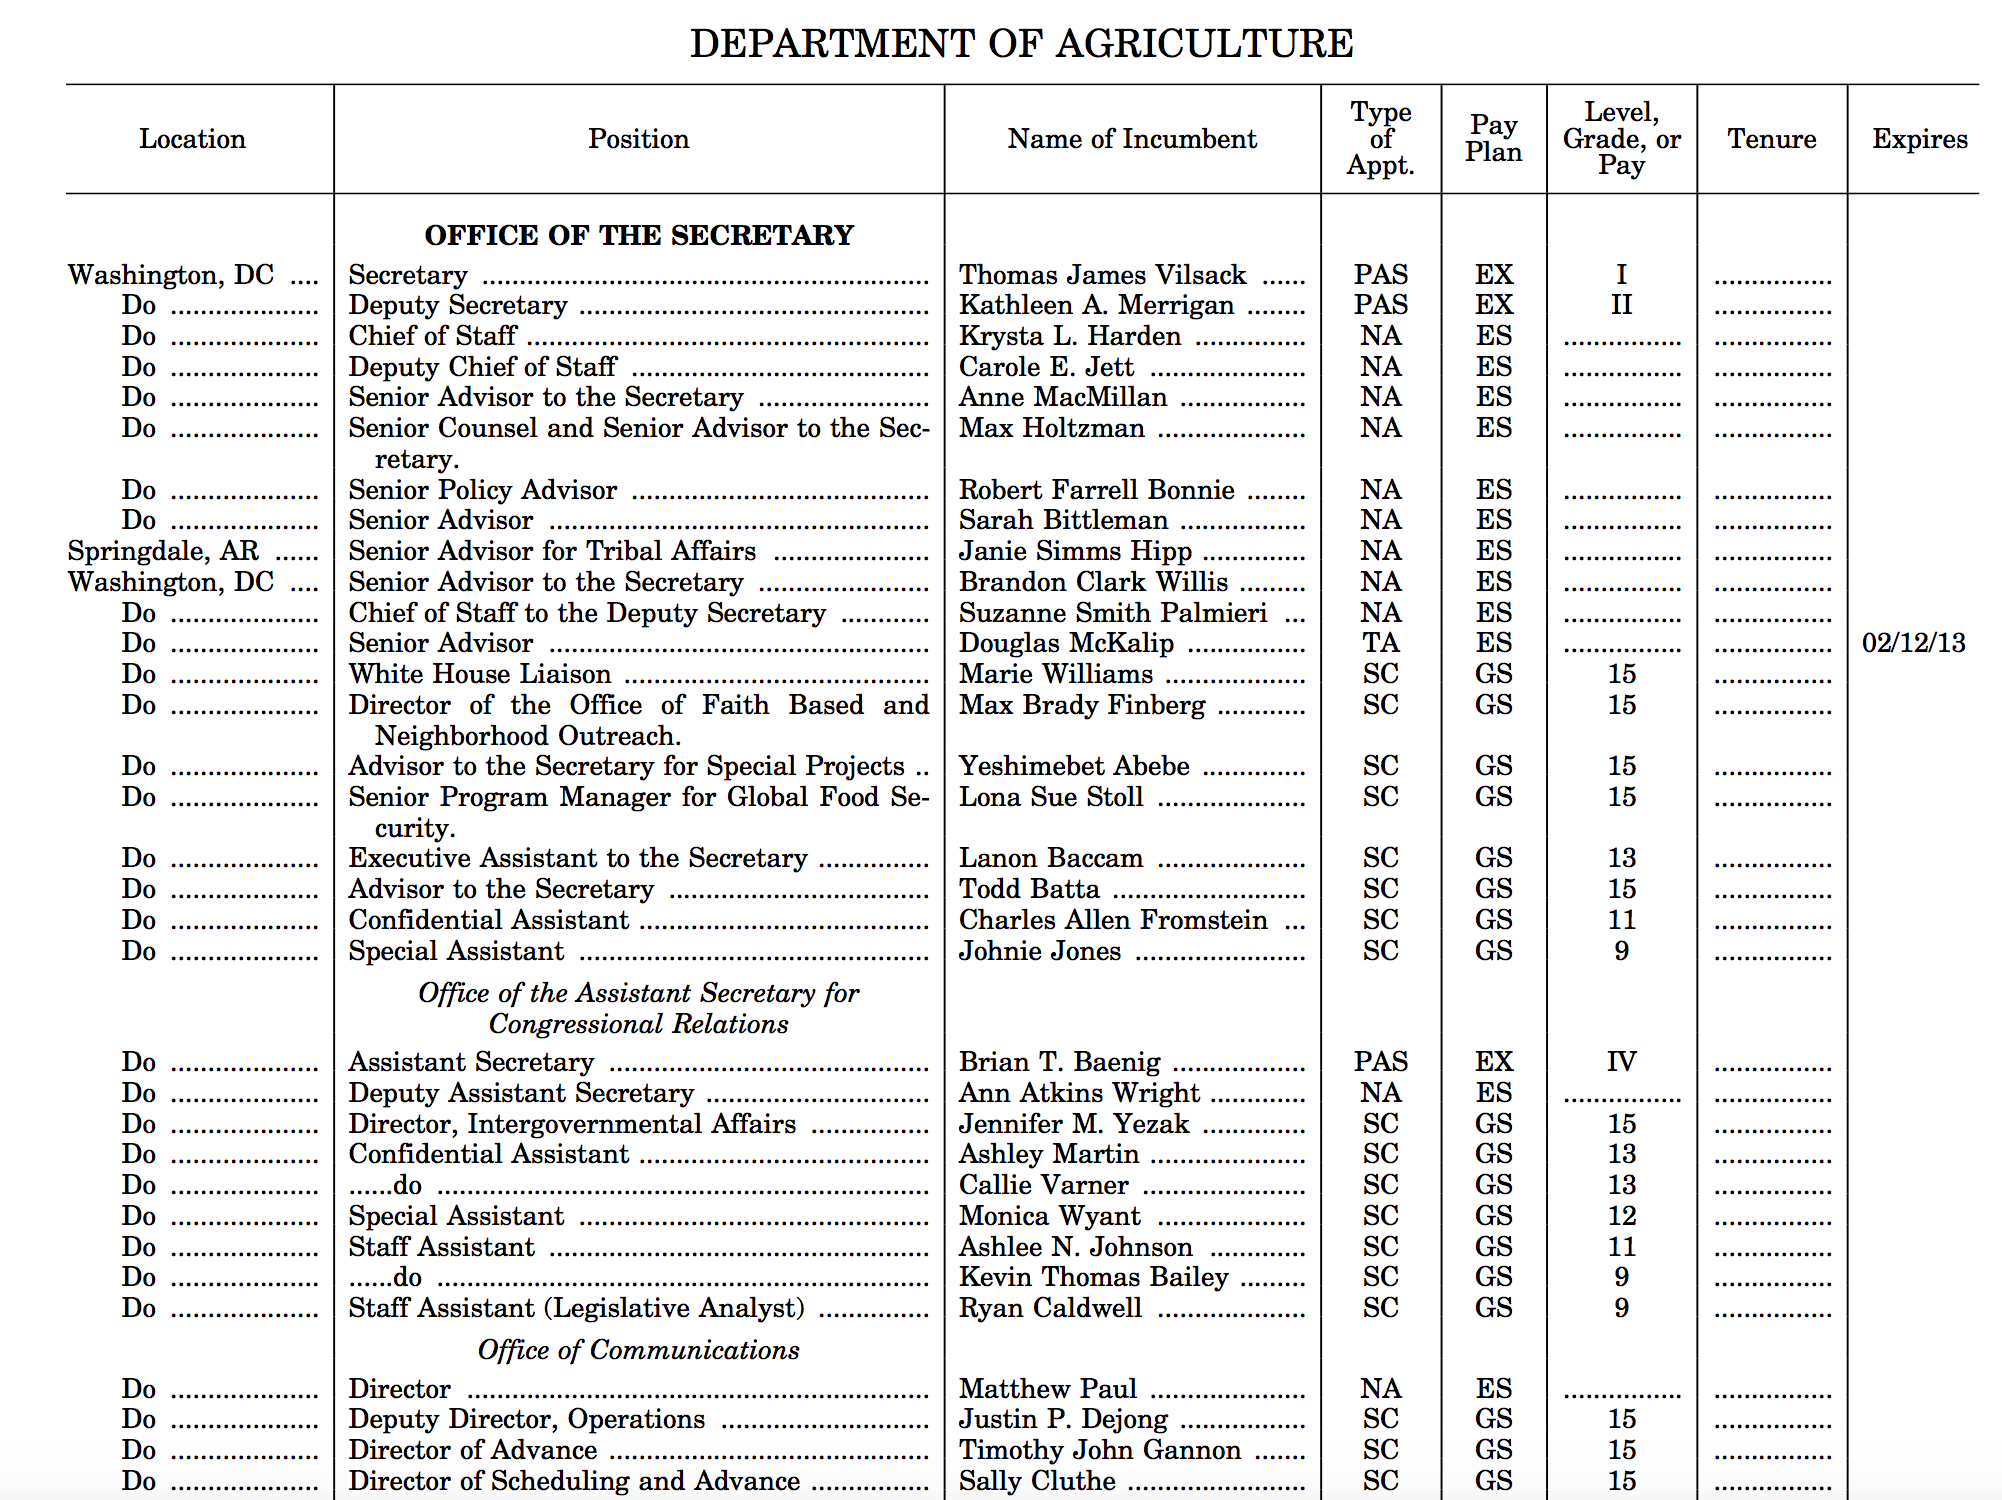
\includegraphics[height=5.5in,width=7in]{PlumBookPage.png}
\caption{Page from the Plum Book on the Department of Agriculture}
\end{center}
\end{figure}

\newpage
\begin{figure}[!htb]
\begin{center}
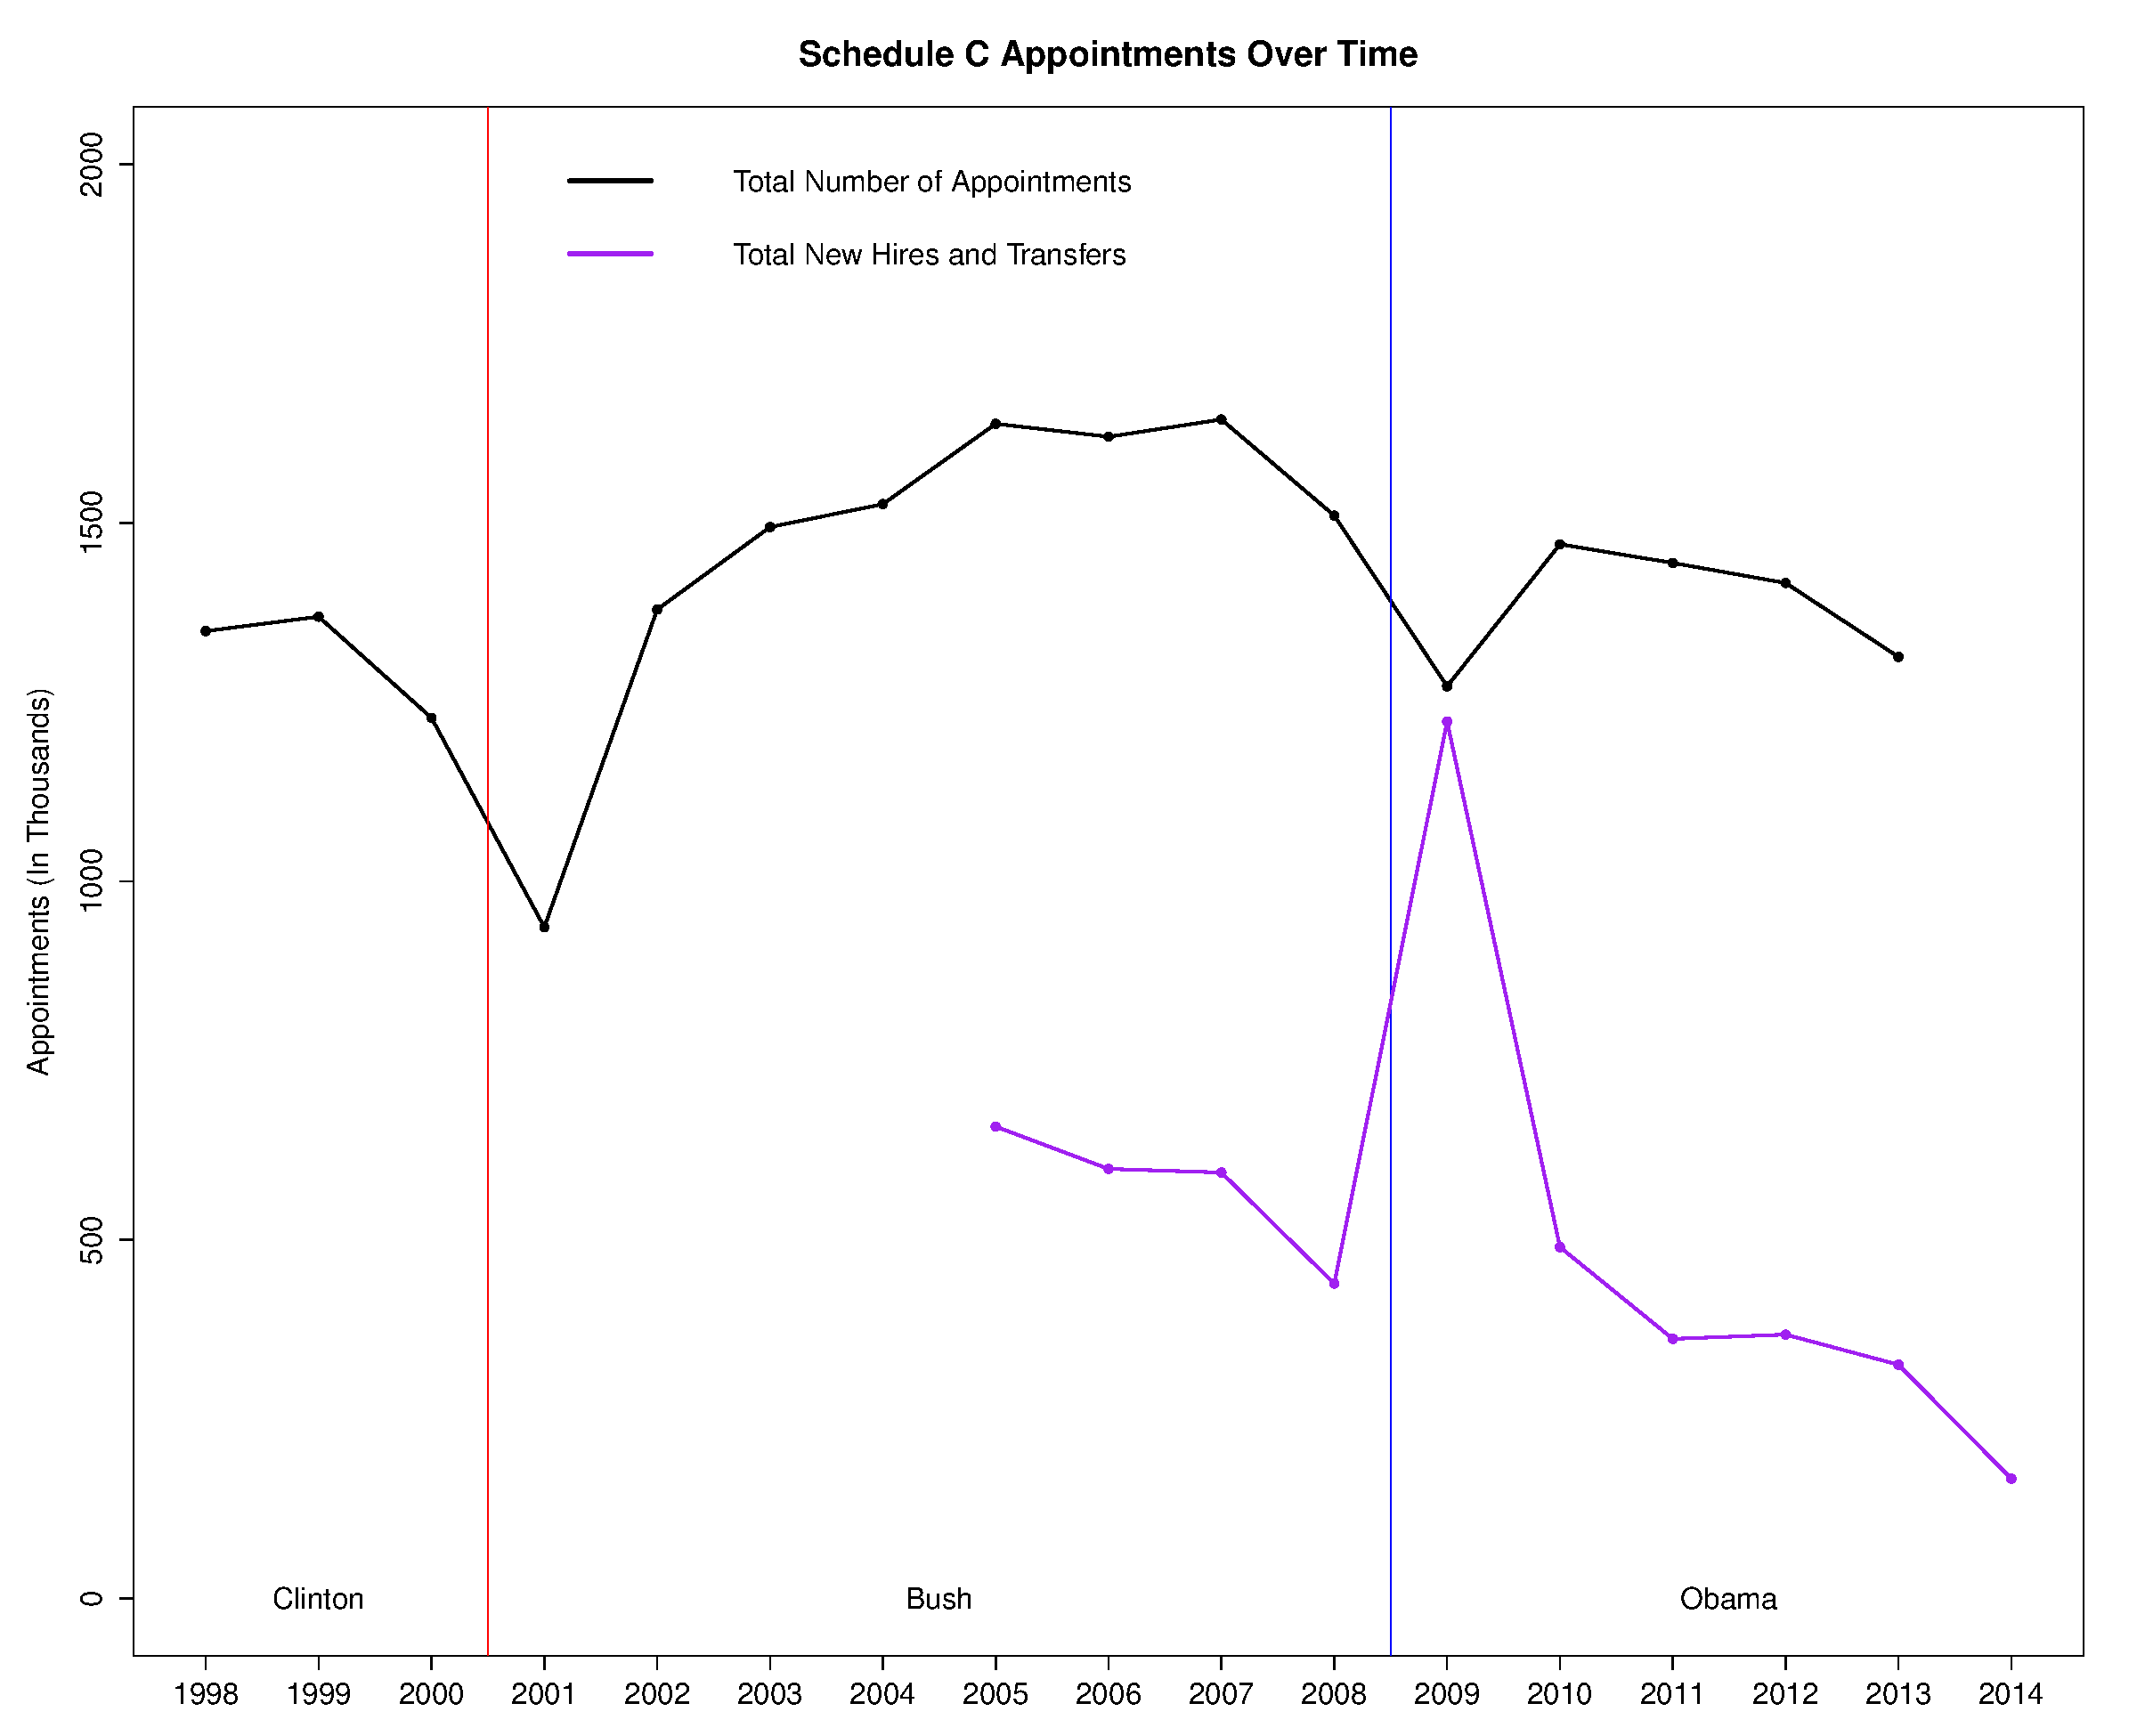
\includegraphics[height=5.5in,width=7in]{SCAptsandAccOverTime.pdf}
\caption{This plot shows the total number of Schedule C appointments over time (black line) in addition to the number of new hires and transfers added to the agency in a given year (purple line).}
\end{center}
\end{figure}

\newpage
\begin{figure}[!h]
\begin{center}
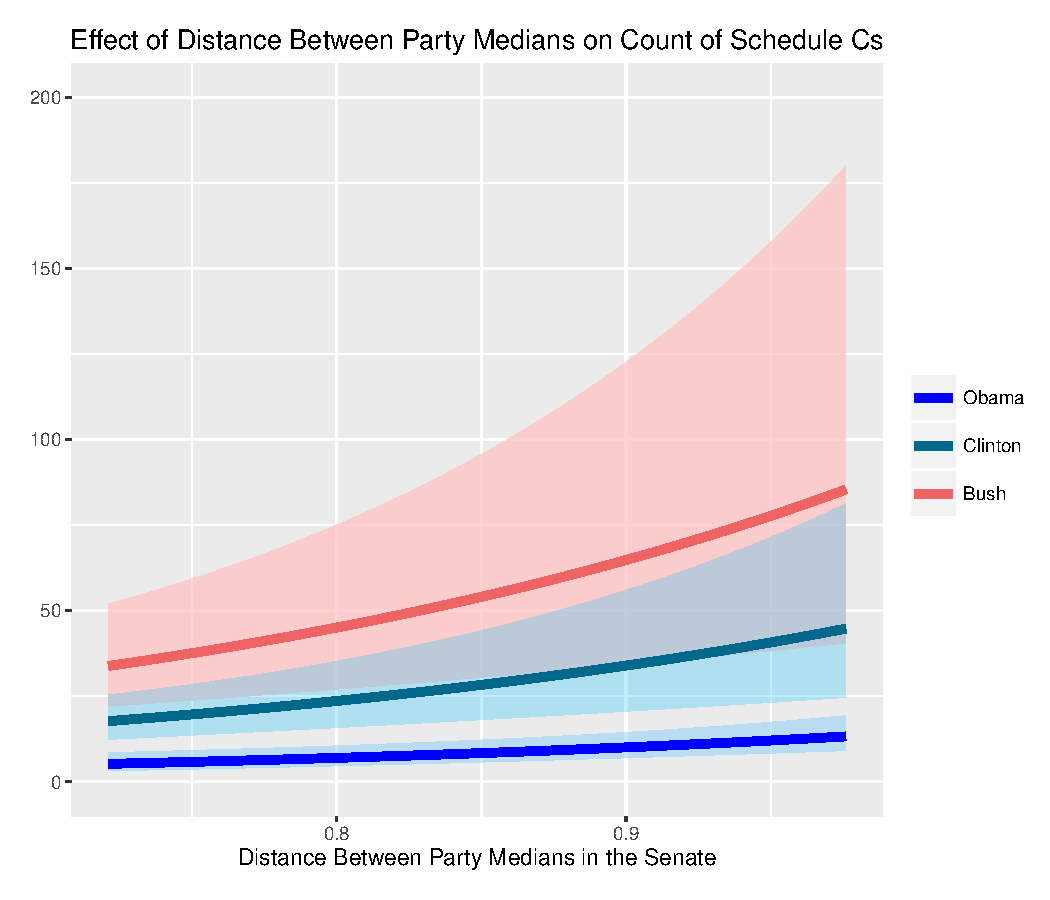
\includegraphics[height=4in,width=4.5in]{ResultsPlots.pdf}
\caption{Predicted Effect of the Ideological Distance Between Party Medians in the Senate on the Number of Schedule C Appointees in an Agency.}
\end{center}
\end{figure}

\newpage
\begin{figure}[!h]
\begin{center}
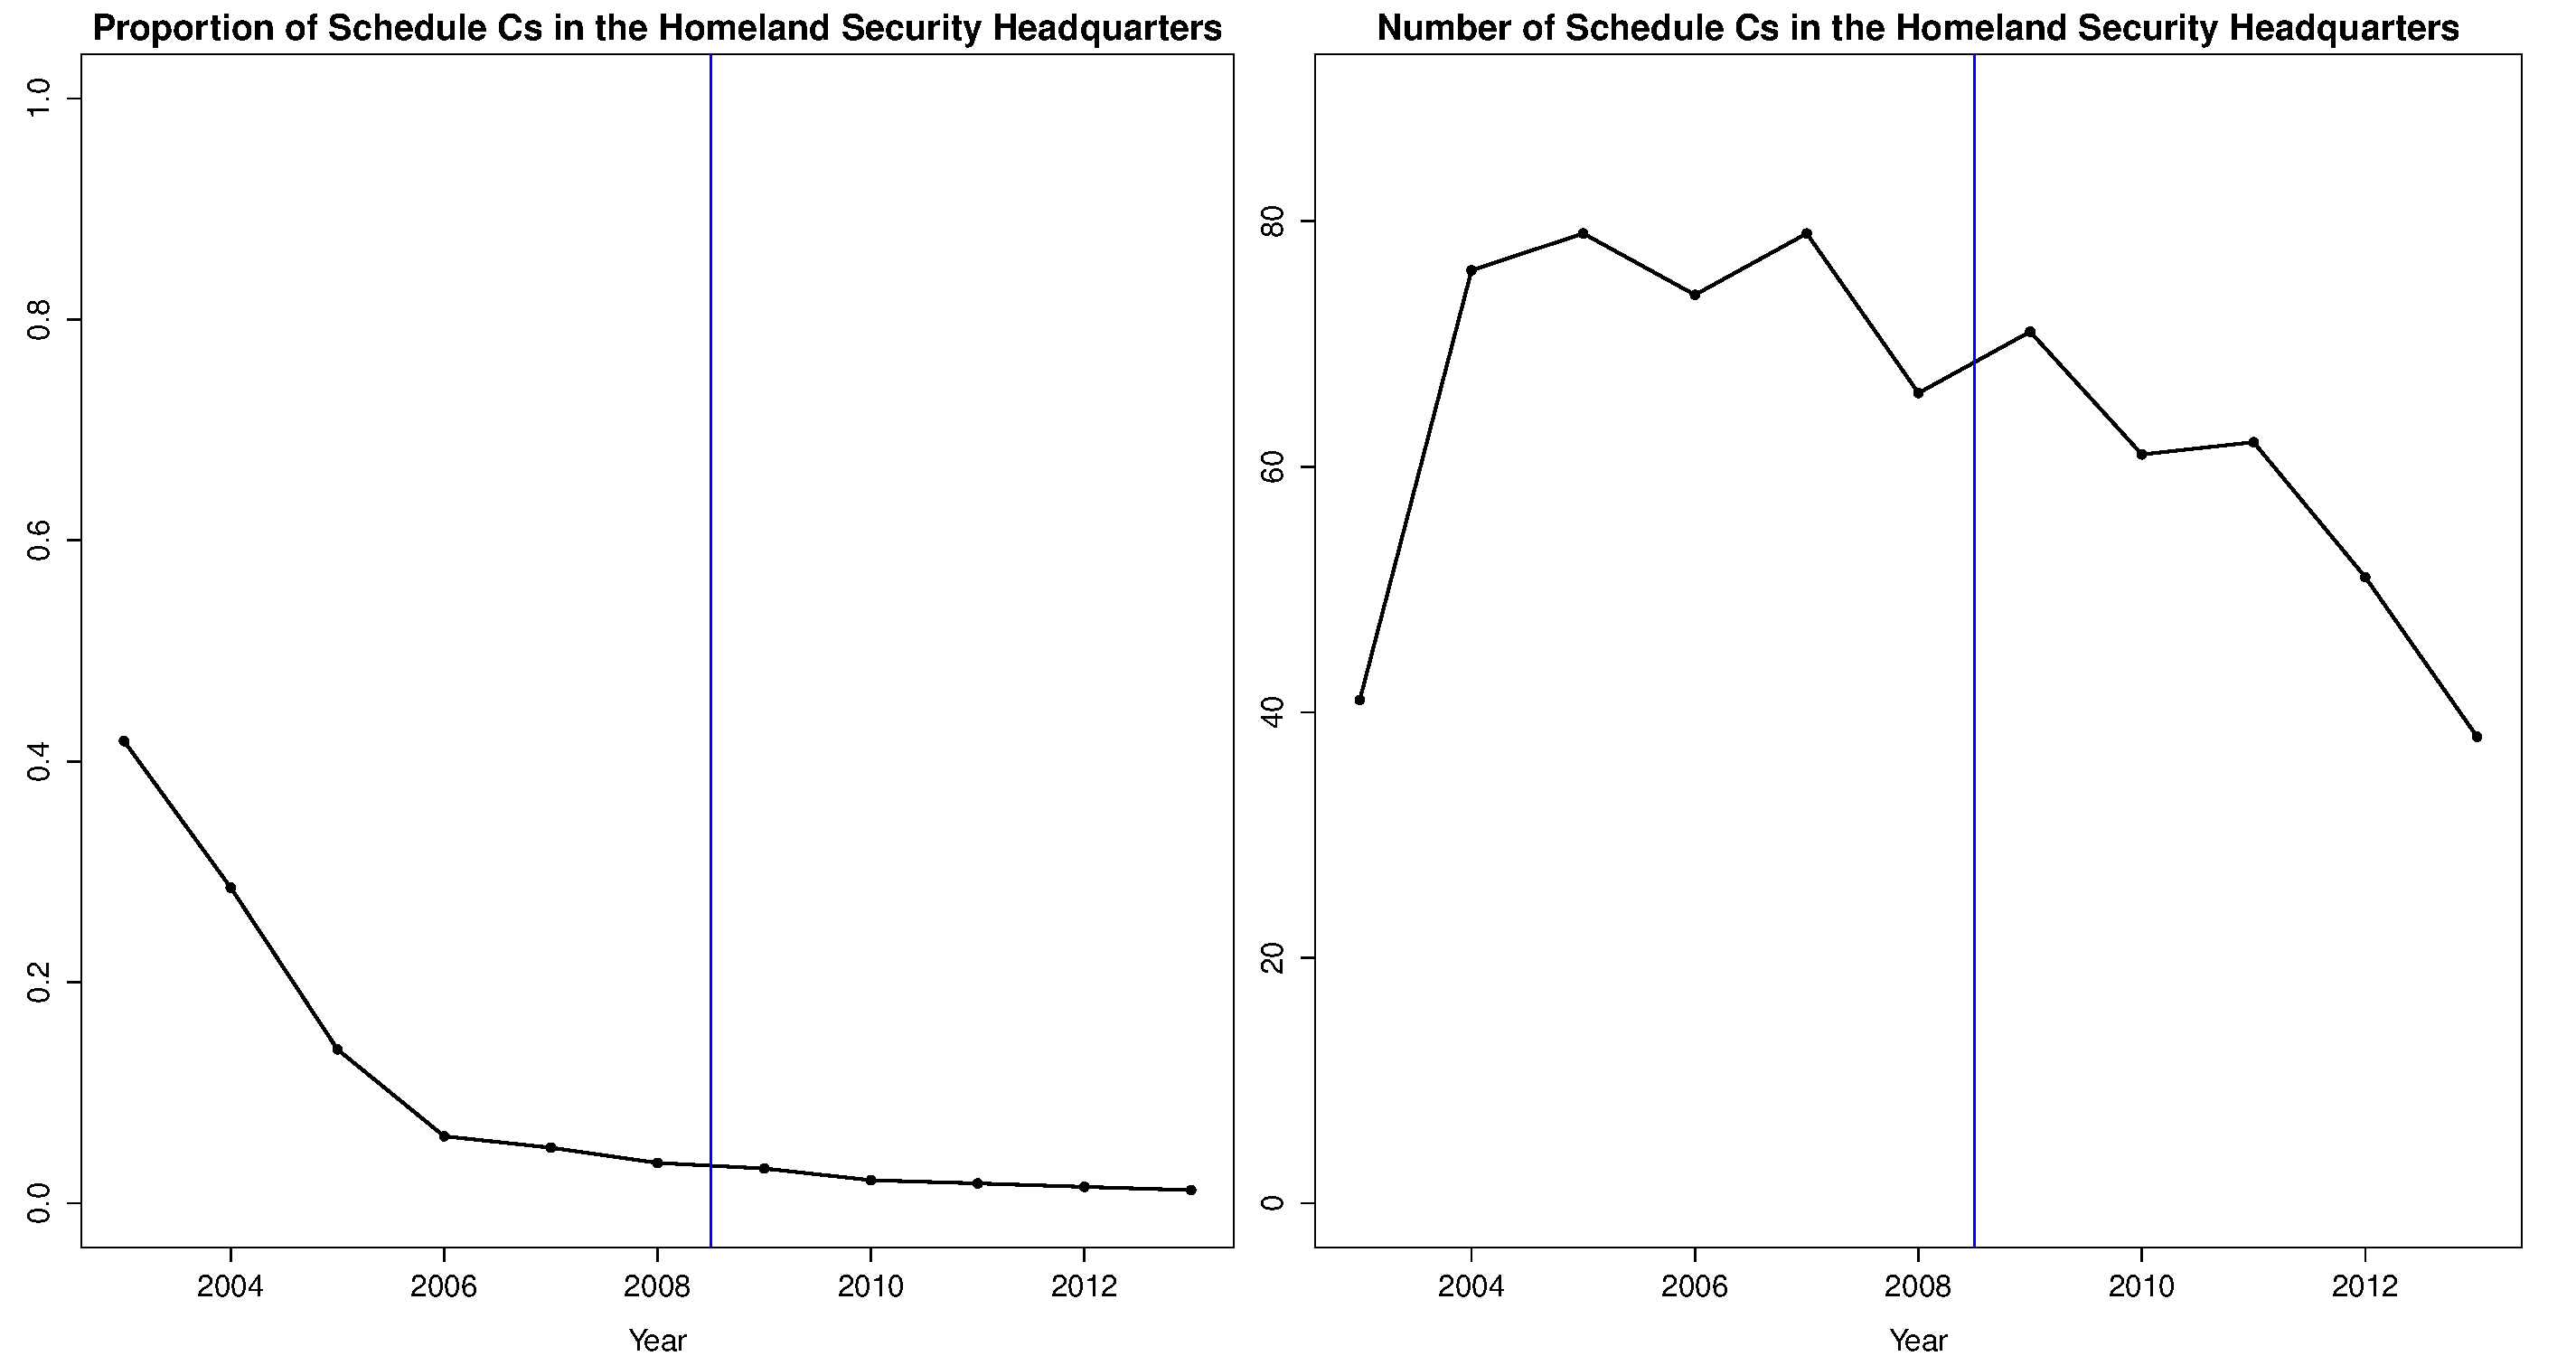
\includegraphics[height=3in,width=6in]{DHSProportionRawNumber.pdf}
\caption{Proportion and Raw Number of Schedule C and Excepted Service Executive Appointments in the Homeland Security Headquarters.}
\end{center}
\end{figure}

\newpage
\section*{Appendix A: Histogram of Dependent Variable: Counts of Schedule Cs.}
\begin{figure}[!h]
\begin{center}
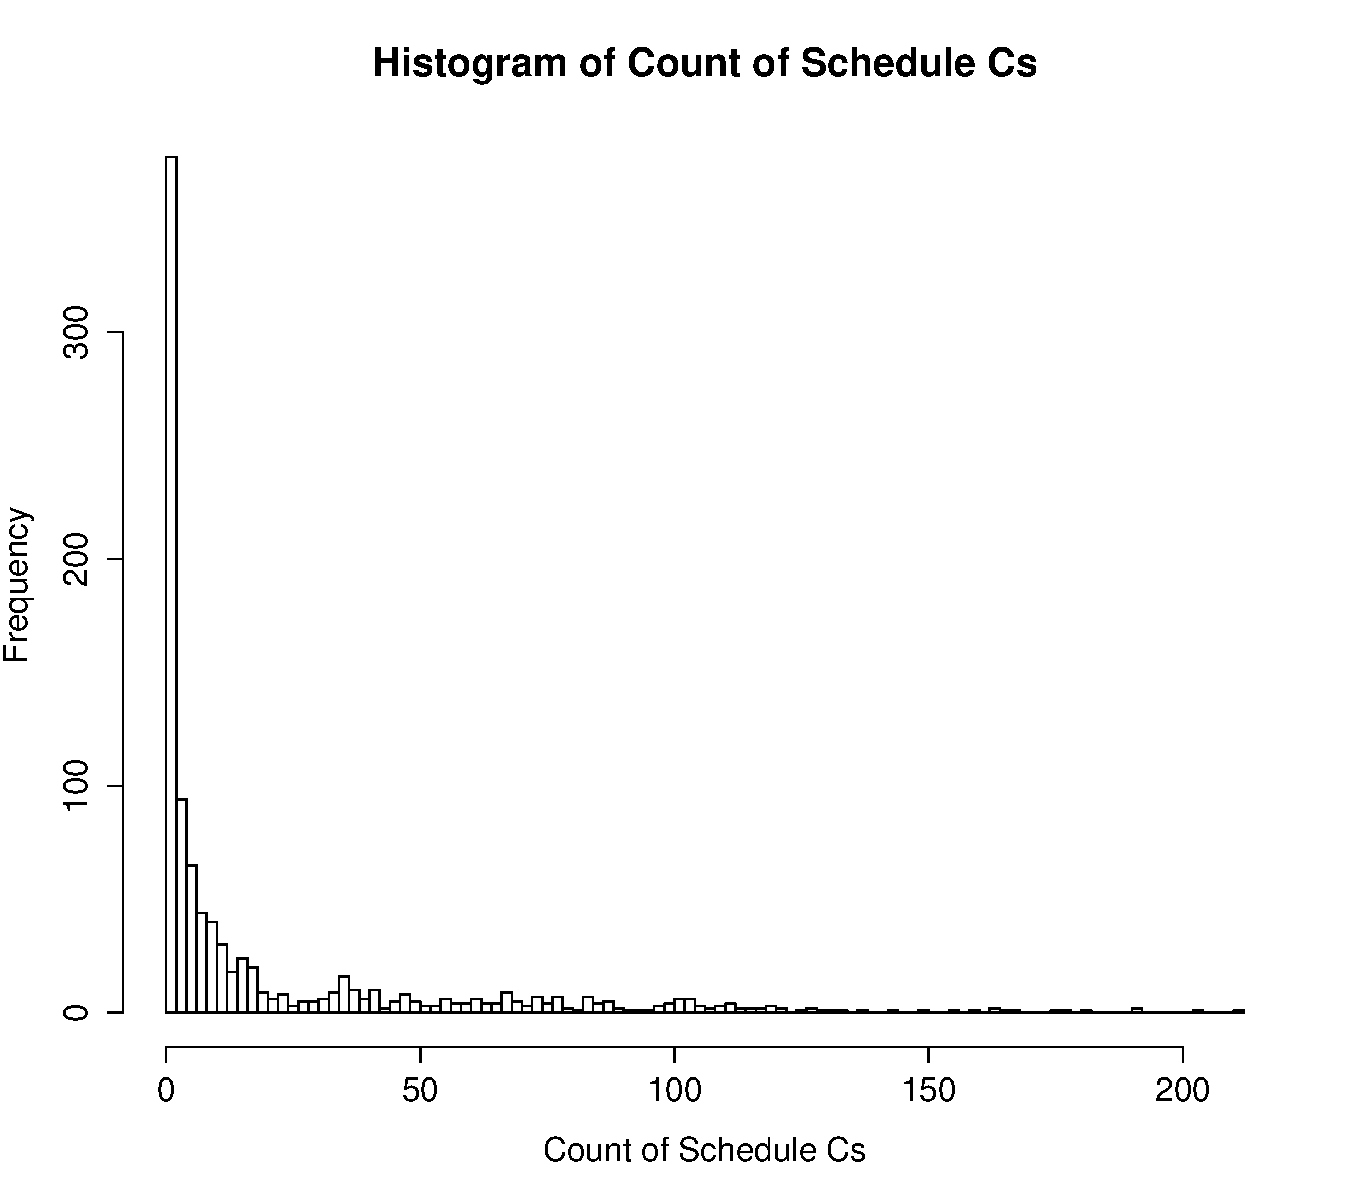
\includegraphics[height=4in,width=5in]{HistogramScheduleCCount.pdf}
\caption{Histogram of Number of Schedule Cs in Agencies.}
\end{center}
\end{figure}




	
%Cooney story	
%	If there is any doubt left over the importance of excepted positions, consider the 2005 Cooney scandal in the Council on Environmental Quality (CEQ). The CEQ formulates reports about the status of environmental resources, reviews the environmental activities of governmental and non-governmental organizations, and oversees the implementation of the environmental impact assessment process. While the CEQ is theoretically designed such that environmental experts assess environmental impact, in reality, the process is often political. Phillip Cooney, who served in an excepted position as CEQ Chief of Staff, had only one qualification relating to the job: he had been employed as a lobbyist for the American Petroleum Institute. In 2005, a scandal broke from a report showing that Cooney purposefully doctored expert-prepared government climate reports to downplay scientific climate change findings. One anonymous EPA employee noted that, for many, Cooney's editing had damaged morale and ``created a sense of frustration'' (Revkin 2005a). The Cooney example exemplifies both the importance of excepted appointments as a political tool to advance the president's interests and the power they are able to wield over policies. 

%Miscellaneous sentences to put in other places:

%It would be easy to conclude that PAS appointees are the only bureaucrats deserving of attention. After all, there is often considerable speculation and controversy surrounding confirmation battles, and these personnel serve in some of the most important positions as cabinet secretaries and heads of independent agencies. 


\end{document}
